\clearpage
\begin{figure}[h]
\begin{center}
\caption{Comparing PTER with PSID \label{inf}}
\includegraphics[width=5in, height=4in]{figure1.eps}
\end{center}
\end{figure}

\newpage

\begin{figure}[h]
\begin{center}
\caption{Comparing PTER with HRS \label{inf}}
\includegraphics[width=5in, height=4in]{figure2.eps}
\end{center}
\end{figure}

\newpage

\begin{figure}[h]
\begin{center}
\caption{Trends of Constrained Workers over Fifty Years \label{inf}}
\includegraphics[width=5in, height=4in]{figure1.eps}
\end{center}
\end{figure}

\newpage

\begin{center}
\footnotesize
\begin{threeparttable}
\caption{Variables Definition and Years Available} \label{Variable}
\label{Variable}
\begin{tabular}{llll}

\hline\hline \\
Definition                                     &PSID                     &     &HRS                     \\
\hline\hline \\
Head Upside Constrained --- Wanted to work     &1967 - 1986              &     &All waves               \\
more hours but were not able to (UC)           &                         &     &                        \\ \\
Head Downside Constrained --- Wanted to        &1967 - 1986              &     &All waves               \\
work fewer hours but were not able to (DC)     &                         &     &                        \\ \\
%Wife Upside Constrained --- Same as head       &1970 - 1975              &     &All waves               \\ \\
Ideal number of market hours                   &NA                       &     &All waves               \\ \\
Hours spent on housework                       &1968 - 1986              &     &NA (off year only)      \\
by head and wife (HWHead, HWWife)              &                         &     &                        \\ \\
Ratio between food consumed out and            &1969 - 1986 except 1973  &     &All waves except 1998   \\
total food expenditure (Food-out ratio)        &                         &     &                        \\ \\
%Number of vacation weeks taken (Weeks)         &1967 - 1986              &     &NA                      \\
\hline\hline \\[-1ex]
\end{tabular}
\begin{tablenotes}
\item[] \footnotesize{The PSID data availabilities refer to the
waves of 1968 -- 1986.  The HRS data have eight waves, every other
year from 1992 to 2006.}
\end{tablenotes}
\label{var}
\end{threeparttable}
\end{center}


\begin{center}
\footnotesize
\begin{threeparttable}
\caption{Summary Statistics} \label{Summary}
\begin{tabular}{lcccccc}
\hline \hline \\[-1ex]
                            &\multicolumn{2}{c}{\underline{Upside Constrained}}
                            &\multicolumn{2}{c}{\underline{Downside Constrained}}
                            &\multicolumn{2}{c}{\underline{Not Constrained}}                      \\[.5em]
                                            &PSID   &HRS      &PSID   &HRS      &PSID   &HRS      \\
                                            & (1)   & (2)     &(3)    & (4)     & (5)   &(6)      \\
\hline \\
\% household $\times$ year                  &18.7   &11.4     &5.7    &8.2      &75.6   &80.5     \\ \\
\% households ever constrained              &52.3   &23.3     &24.8   &17.1     &35.8   &62.5     \\ \\
By how many hours                           &NA     &451      &NA     &731      &NA     &NA       \\
                                            &       &(323)    &       &(440)    &       &         \\
Demographic Characteristics &&&&&& \\
\hspace{.3in} Age                           &37.6   &56.3     &41.3   &57.1     &40.9   &57.6     \\
                                            &(11.2) &(4.5)    &(12.0) &(4.3)    &(12.1) &(4.9)    \\[1ex]
\hspace{.3in} White (\%)                    &80.2   &81.5     &88.9   &86.9     &88.9   &87.0     \\[1ex]
\hspace{.3in} Below high school (\%)        &34.3   &13.6     &23.0   &9.0      &22.6   &11.4     \\[1ex]
\hspace{.3in} High school graduate (\%)     &38.6   &30.6     &36.3   &32.5     &33.3   &27.3     \\[1ex]
\hspace{.3in} Some college and college (\%) &27.1   &55.9     &40.7   &58.3     &44.1   &61.3     \\[1ex]
\hspace{.3in} Married (\%)                  &73.7   &61.7     &72.9   &65.6     &73.8   &68.9     \\ \\

Income (1986 dollars)and hours worked       &       &         &       &         &       &         \\
\hspace{.3in} Family income(\$thousands)    &29.3   &35.9     &40.5   &47.8     &39.5   &52.8     \\
                                            &(17.3) &(31.9)   &(24.3) &(45.9)   &(25.7) &(61.7)   \\[1ex]
\hspace{.3in} Hours worked                  &1,968  &2,022    &2,301  &2,299    &2,180  &2,144    \\
                                            &(525)  &(487)    &(566)  &(479)    &(610)  &(559)    \\
\hspace{.3in} Working part time             &28.2   & 22.3    &12.9   & 8.2     &19.2   & 25.2    \\ \\

Home production                             &       &         &       &         &       &         \\
\hspace{.3in} Unmarried head housework hours&629    &NA       &539    &NA       &559    &NA       \\
                                            &(471)  &         &(425)  &         &(443)  &         \\[1ex]
\hspace{.3in} Married head housework hours  &326    &NA       &292    &NA       &291    &NA       \\
                                            &(383)  &         &(342)  &         &(342)  &         \\[1ex]
\hspace{.3in} Married wife housework hours  &1,385  &NA       &1,469  &NA       &1,420  &NA       \\
                                            &(799)  &         &(781)  &         &(781)  &         \\[1ex]
\hspace{.3in} Unmarried food-out ratio (\%) &25.5   &18.3     &31.5   &22.8     &31.2   &22.0     \\[1ex]
\hspace{.3in} Married food-out ratio (\%)   &14.3   &18.8     &18.1   &22.9     &17.8   &22.1     \\[1ex]
%\hspace{.3in} Wife housework hours          &1,490  &NA       &1,490  &NA       &1,460  &NA       \\
%                                            &(843)  &         &(833)  &         &(829)  &         \\[1ex]
\hline\hline \\[-1ex]
\end{tabular}
\begin{tablenotes}
\item[] \footnotesize{All statistics are computed using the PSID
and HRS weights. Standard deviations of continuous variables are
reported in parenthesis.}
\end{tablenotes}
\label{sum}
\end{threeparttable}
\end{center}

\clearpage

\begin{center}
\scriptsize
\begin{threeparttable}
\caption{Occupation and Industry} \label{OCCIND}
\begin{tabular}{lcclcclcclc}
\hline \hline \\[-1ex]
                            \multicolumn{5}{c}{Occupation} &&\multicolumn{5}{c}{Industry} \\
                            (1) & (2) && (3) & (4) \\[.5em]
\hline\\[-1ex]
                            \multicolumn{2}{c}{\underline{Upside}}&&\multicolumn{2}{c}{\underline{Downside}}&&\multicolumn{2}{c}{\underline{Upside}}&&\multicolumn{2}{c}{\underline{Downside}} \\
                            Laborers				  		& 32.5	&&	Farm laborers	    &	6.9         && Construction	        & 29.3    &&    Mining	             & 7.7 \\[1ex]
                            Operatives						& 30.0  &&  Operatives	        &	6.3         && Entertainment     	& 26.0    &&    Manufacturing	     & 6.7 \\[1ex]
                            Trans. operators   		        & 27.1  &&  Craftsman	        &	6.2         && Personal Services    & 23.3    &&    Public Admin	     & 6.3 \\[1ex]
                            Farm laborers					& 24.7  &&  Trans. operators    &	6.0         && Manufacturing	    & 20.7    &&    Trans., Comm., Util. & 6.2 \\[1ex]
                            Service workers				    & 23.4  &&  Manager	            &	6.0         && Trans., Comm., Util.	& 20.0    &&    Wholesale and Retail & 5.7 \\[1ex]
                            Craftsman						& 23.0  &&  Professional	    &	6.0         && Business and Repair  & 18.2    &&    Business and Repair	 & 5.3 \\[1ex]
                            Clerical						& 21.3  &&  Clerical      	    &	5.4         && Mining	            & 16.7    &&    Agriculture	         & 4.7 \\[1ex]
                            Priv. hhld. workers  	        & 19.1  &&  Service workers	    &	5.4         && Public Admin.       	& 16.3    &&    Construction	     & 4.6 \\[1ex]
                            Sales							& 11.6  &&  Farmers	            &	3.2         && Wholesale and Retail	& 16.1    &&    Professional	     & 4.5 \\[1ex]
                            Professional					& 11.2  &&  Sales	            &	3.2         && Professional	        & 13.5    &&    Personal Services	 & 4.5 \\[1ex]
                            Manager							& 7.5   &&  Laborers	        &	3.0         && Agriculture	        & 11.6    &&    Finance	             & 4.2 \\[1ex]
                            Farmers							& 5.3   &&  Priv. hhld workers  &	1.5         && Finance              & 10.2    &&    Entertainment	     & 2.3 \\
\hline\hline \\[-1ex]
\end{tabular}
\begin{tablenotes}
\item[] All statistics are computed using the PSID weights.
\end{tablenotes}
\label{sum}
\end{threeparttable}
\end{center}

\begin{center}
\footnotesize
\begin{threeparttable}
\caption{Transition Matrix of Constraint Status} \label{Markov}
\begin{tabular}{lccc}
\hline \hline \\[-1ex]
\multicolumn{4}{c}{Panel A Overall Transition Matrix (\%)} \\
\hline \\[-1ex]
                          & \multicolumn{3}{c}{Year t+1}  \\
Year t                    & Upside constrained &  Unconstrained & Downside constrained \\ \\
Upside constrained        &  48.2              &  49.2          & 2.6                  \\ \\
Unconstrained             &  11.1              &  84.2          & 4.7                  \\ \\
Downside constrained      &  7.6               &  62.3          & 30.1                 \\
\hline \\[-1ex]
\end{tabular}

\begin{tabular}{lccccc}
\multicolumn{6}{c}{Panel B Upside Constraint Transitions by Part-Time Status (\%)} \\
\hline \\[-1ex]
                          & \multicolumn{2}{c}{Full-time only}  && \multicolumn{2}{c}{Part-time only}\\
\cline{2-3} \cline{5-6}

                          & Constrained &  Unconstrained && Constrained & Unconstrained \\ \\
Constrained               &  52.9       &  47.2          && 55.9        & 44.1          \\ \\
Unconstrained             &  9.8        &  90.2          && 12.9        & 87.1          \\ \\

                          & \multicolumn{2}{c}{Full-time to part-time}  && \multicolumn{2}{c}{Part-time to full-time}\\
\cline{2-3} \cline{5-6}

                          & Constrained &  Unconstrained && Constrained & Unconstrained \\ \\
Constrained               &  49.3       &  50.7          && 42.4        & 57.6          \\ \\
Unconstrained             &  17.7       &  82.3          && 11.5        & 88.5          \\ \\
\hline
\end{tabular}

\begin{tabular}{lccccc}
\multicolumn{6}{c}{Panel C Subsequent-Year Status of the Upside Constrained (\%)} \\
\hline \\[-1ex]
                          & \multicolumn{5}{c}{Year t+1}\\
\cline{2-6}

                          & \multicolumn{2}{c}{Full-time} && \multicolumn{2}{c}{Part-time}  \\
Year t                    & Constrained &  Unconstrained  && Constrained & Unconstrained \\ \\
Full-time                 & 40.3        &  45.2           && 7.1         & 7.3          \\ \\
Part-time                 & 31.5        &  24.8           && 18.5        & 25.2          \\ \\
\hline
\end{tabular}
\begin{tablenotes}
\item[] \footnotesize{All statistics are computed using the PSID weights.}
\end{tablenotes}
\label{sum}
\end{threeparttable}
\end{center}

\clearpage

\begin{center}
\footnotesize
\begin{threeparttable}
\caption{Factors Associated with Transitions into and out of Constraints} \label{TransitionReg}
\begin{tabular}{lccccc}
\hline \hline \\[-1ex]
                          &\multicolumn{2}{c}{Became upside constrained} && \multicolumn{2}{c}{Escaped upside constraints}\\
                          & (1)           & (2)           &&      (3)      & (4)           \\
Head characteristics      &&&&&\\[1ex]
\hspace{.1in}Black                     &       1.724***&       1.399***&&       0.899** &       1.000   \\
                                       &     (0.071)   &     (0.069)   &&     (0.040)   &     (0.053)   \\
\hspace{.1in}High school               &       0.671***&       0.713***&&       1.121** &       1.091   \\
                                       &     (0.031)   &     (0.039)   &&     (0.058)   &     (0.066)   \\
\hspace{.1in}Some college              &       0.497***&       0.594***&&       1.385***&       1.273***\\
                                       &     (0.030)   &     (0.044)   &&     (0.096)   &     (0.103)   \\
\hspace{.1in}College                   &       0.262***&       0.446***&&       1.791***&       1.468***\\
                                       &     (0.019)   &     (0.050)   &&     (0.172)   &     (0.186)   \\
Lifecycle events                       &               &               &&               &               \\[1ex]
\hspace{.1in}Became homeowner          &       1.090   &       1.120   &&       0.983   &       0.955   \\
                                       &     (0.073)   &     (0.095)   &&     (0.081)   &     (0.092)   \\
\hspace{.1in}Got married               &       0.909   &       0.787   &&       1.019   &       0.994   \\
                                       &     (0.116)   &     (0.129)   &&     (0.147)   &     (0.165)   \\
\hspace{.1in}Remain married            &       1.185***&       1.246***&&       0.868***&       0.895*  \\
                                       &     (0.053)   &     (0.068)   &&     (0.043)   &     (0.054)   \\
\hspace{.1in}Divorced/Separated        &       1.004   &       0.985   &&       1.196   &       1.317   \\
                                       &     (0.122)   &     (0.152)   &&     (0.179)   &     (0.231)   \\
\hspace{.1in}Change number of children &       1.174***&       1.263***&&       0.954   &       1.039   \\
                                       &     (0.062)   &     (0.082)   &&     (0.057)   &     (0.074)   \\
Income and employment                  &               &               &&&\\[1ex]
\hspace{.1in}Change log(faminc)        &       0.559***&       0.575***&&       1.394***&       1.429***\\
                                       &     (0.032)   &     (0.046)   &&     (0.093)   &     (0.122)   \\
\hspace{.1in}Change log(wage)          &       1.191***&       1.251***&&       0.860** &       0.895   \\
                                       &     (0.063)   &     (0.092)   &&     (0.052)   &     (0.073)   \\
\hspace{.1in}F.T. to P.T.              &       1.695***&       1.503***&&       1.042   &       1.067   \\
                                       &     (0.082)   &     (0.091)   &&     (0.063)   &     (0.077)   \\
\hspace{.1in}P.T. to F.T.              &       1.221***&       1.109   &&       1.100   &       1.096   \\
                                       &     (0.076)   &     (0.086)   &&     (0.064)   &     (0.077)   \\
\hspace{.1in}P.T. to P.T.              &       1.606***&       1.472***&&       0.714***&       0.753*** \\
                                       &     (0.091)   &     (0.110)   &&     (0.041)   &     (0.054)    \\
\hspace{.1in}Changed jobs              &               &               &&       1.237***&       1.251*** \\
                                       &               &               &&     (0.058)   &     (0.071)    \\
\hspace{.1in}Got additional job        &               &               &&       1.045   &       1.092    \\
                                       &               &               &&     (0.066)   &     (0.084)    \\
Controlled for                         &               &               &&               &               \\[1ex]
\hspace{.1in} Head age polynomial      & Yes           & Yes           &&  Yes          &  Yes          \\
\hspace{.1in} Year fixed effects       & Yes           & Yes           &&  Yes          &  Yes          \\[1ex]
Pseudo R-squared                       & 0.066         & 0.038         &&  0.020        &  0.014        \\
N                                      &       41,353  &       20,114  &&      13,671   &       9,247   \\ \hline
\end{tabular}
\begin{tablenotes}
\item[] \footnotesize{}
\end{tablenotes}
\label{sum}
\end{threeparttable}
\end{center}

\clearpage

\begin{center}
\begin{threeparttable}
\caption{Effects of Market Work Hours Constraints on Singles' Housework Hours} \label{Single}
\begin{footnotesize}
\begin{tabular}{lccccccc}
\hline \hline
                     & \multicolumn{3}{c}{Whole sample}  && \multicolumn{3}{c}{Can get extra pay} \\
\cline{2-4} \cline{6-8} \\
                     &OLS            &Tobit          &Panel          &&OLS            &Tobit          &Panel           \\
                     &(1)            &(2)            &(3)            &&(5)            &(6)            &(7)             \\
\hline \\
Upside Constrained   &        46.5***&        47.6***&        26.3***&&        56.1***&        57.5***&        29.1**  \\
                     &      (11.7)   &      (10.1)   &      (10.0)   &&      (14.1)   &      (12.9)   &      (14.1)    \\
Downside Constrained &        -3.6   &        -5.8   &       -13.1   &&       -13.9   &       -18.8   &        -5.4    \\
                     &      (19.1)   &      (18.4)   &      (17.6)   &&      (23.3)   &      (23.7)   &      (24.2)    \\
Black                &        34.5** &        36.2***&               &&        36.0** &        38.6***&                \\
                     &      (15.2)   &       (9.4)   &               &&      (17.6)   &      (12.1)   &                \\
High school          &       -21.1   &       -16.6   &               &&        -7.6   &        -0.2   &                \\
                     &      (17.6)   &      (11.1)   &               &&      (20.4)   &      (14.3)   &                \\
Some college         &       -59.3***&       -52.5***&               &&       -46.6** &       -37.4** &                \\
                     &      (20.4)   &      (13.4)   &               &&      (22.7)   &      (17.3)   &                \\
College              &      -114.2***&      -106.3***&               &&       -76.5** &       -64.2***&                \\
                     &      (23.0)   &      (14.7)   &               &&      (30.3)   &      (24.0)   &                \\
Number of children   &        86.7***&        85.9***&        39.9***&&        89.9***&        89.0***&        39.2*** \\
                     &       (9.0)   &       (4.1)   &       (6.2)   &&      (10.1)   &       (5.6)   &       (8.9)    \\
Number of adults     &       -14.0   &       -22.8***&        -4.0   &&       -12.2   &       -19.0** &         5.8    \\
                     &      (10.7)   &       (6.5)   &       (8.5)   &&      (13.7)   &       (9.1)   &      (13.1)    \\
Single female        &       236.8***&       269.7***&               &&       223.6***&       253.8***&                \\
                     &      (14.6)   &       (9.6)   &               &&      (18.5)   &      (13.1)   &                \\
Working part-time    &        57.2***&        61.1***&        24.9** &&        47.6***&        49.9***&        15.6    \\
                     &      (11.7)   &       (9.2)   &       (9.7)   &&      (14.9)   &      (12.6)   &      (14.1)    \\
N                    &       13,451  &       13451   &       13,451  &&        7,038  &        7,038  &        7,038   \\

\hline\hline
\end{tabular}
\end{footnotesize}
\begin{tablenotes}
\item[] \footnotesize{\noindent 90\% 95\% and 99\% statistical
significance are denoted by *, ** and ***, respectively.}
\end{tablenotes}
\label{Analysis}
\end{threeparttable}
\end{center}

\clearpage
\begin{landscape}
\begin{center}
\begin{threeparttable}
\caption{Effects of Market Work Hours Constraints on Married Households} \label{Married}
\begin{footnotesize}
\begin{tabular}{lcccccccccccc}
\hline \hline
                     & \multicolumn{5}{c}{Housework hours}  && \multicolumn{6}{c}{Wife work status} \\
\cline{2-6} \cline{8-13} \\
                     & \multicolumn{2}{c}{\underline{Head}} && \multicolumn{2}{c}{\underline{Wife}}  && \multicolumn{2}{c}{\underline{Extensive margin}} && \multicolumn{3}{c}{\underline{intensive margin}} \\
                     &               &               &&               &               && Work          & Start to work && Work part-time& Work hours    & Work hours \\
                     &Tobit          &Panel FE       && Tobit         & Panel FE      && Logistic      & Logistic      && Logistic      & OLS           & Panel FE      \\
                     &(1)            &(2)            &&(3)            &(4)            &&(5)            &(6)            && (7)           & (8)           & (9)   \\
\hline \\[-1ex]
Upside Constrained   &       30.68***&       10.41** &&       -24.7** &       -16.4   &&       1.22***&        1.16** &&        0.92*  &       53.48***&       36.52***\\
                     &      (6.79)   &      (5.30)   &&      (10.7)   &      (10.7)   &&     (0.05)   &      (0.07)   &&      (0.04)   &     (15.50)   &     (11.52)   \\
Down Constrained     &      -11.48   &       -9.28   &&        35.1*  &        14.6   &&       0.96   &        1.11   &&        1.21***&      -15.77   &      -16.21   \\
                     &     (12.31)   &      (9.12)   &&      (19.3)   &      (18.4)   &&     (0.06)   &      (0.13)   &&      (0.09)   &     (27.40)   &     (19.94)   \\
Black                &       68.26***&               &&      -310.5***&               &&       1.72***&        1.26***&&        0.56***&      262.99***&               \\
                     &      (6.76)   &               &&      (10.6)   &               &&     (0.10)   &      (0.09)   &&      (0.03)   &     (20.51)   &               \\
Head Education       &               &               &&           .   &               &&              &               &&               &               &               \\
\;\;\;High school    &       57.40***&               &&        68.2***&               &&       0.81***&        0.90   &&        1.47***&     -114.63***&               \\
                     &      (7.71)   &               &&      (11.9)   &               &&     (0.05)   &      (0.07)   &&      (0.10)   &     (25.56)   &               \\
\;\;\;Some college   &      102.37***&               &&        41.7***&               &&       0.79***&        0.95   &&        1.64***&     -180.12***&               \\
                     &      (9.41)   &               &&      (14.8)   &               &&     (0.06)   &      (0.09)   &&      (0.14)   &     (30.31)   &               \\
\;\;\;College        &      102.79***&               &&        56.8***&               &&       0.59***&        0.87   &&        2.52***&     -324.47***&               \\
                     &     (10.37)   &               &&      (16.4)   &               &&     (0.05)   &      (0.09)   &&      (0.24)   &     (34.27)   &               \\
Wife Education       &               &               &&           .   &               &&              &               &&               &               &               \\
\;\;\;High school    &       35.05***&               &&        16.1   &               &&       1.07   &        1.01   &&        0.96   &       -0.92   &               \\
                     &      (8.85)   &               &&      (13.5)   &               &&     (0.07)   &      (0.09)   &&      (0.07)   &     (28.70)   &               \\
\;\;\;Some college   &       75.37***&               &&       -67.2***&               &&       1.43***&        1.41***&&        0.94   &       -1.82   &               \\
                     &      (9.31)   &               &&      (14.4)   &               &&     (0.10)   &      (0.13)   &&      (0.07)   &     (28.62)   &               \\
\;\;\;College        &       71.86***&               &&      -146.5***&               &&       2.07***&        1.39** &&        1.60***&      -73.87** &               \\
                     &     (12.33)   &               &&      (19.5)   &               &&     (0.21)   &      (0.19)   &&      (0.16)   &     (36.17)   &               \\
Num. children        &       -5.68** &       -3.14   &&       150.4***&       122.8***&&       0.83***&        0.91***&&        1.23***&      -70.96***&      -57.06***\\
                     &      (2.24)   &      (2.19)   &&       (3.4)   &       (4.4)   &&     (0.01)   &      (0.02)   &&      (0.02)   &      (7.27)   &      (5.11)   \\
Num. adults          &      -35.52***&       -6.67   &&        62.6***&        57.0***&&       0.87***&        0.88***&&        1.13***&      -71.88***&     -101.09***\\
                     &      (4.96)   &      (4.30)   &&       (7.5)   &       (8.7)   &&     (0.03)   &      (0.04)   &&      (0.05)   &     (16.49)   &      (9.51)   \\
Work part time       &       45.98***&       13.76** &&      -112.7***&       -55.4***&&       1.32***&        1.12   &&        0.92*  &       80.45***&       56.89***\\
                     &      (7.75)   &      (6.24)   &&      (12.2)   &      (12.6)   &&     (0.06)   &      (0.08)   &&      (0.05)   &     (17.67)   &     (13.66)   \\
N                    &       30,743  &       30,743  &&       30,743  &       30,743  &&      38,337  &       11,031  &&       24,960  &       20,740  &       22,141  \\\hline\hline
\end{tabular}
\end{footnotesize}
\end{threeparttable}
\end{center}
\end{landscape}

\newpage
\begin{center}
\begin{threeparttable}
\caption{Market Hours Constraints and Food-Out Shares } \label{HRS}
\begin{footnotesize}
\begin{tabular}{lccccccccc}
\hline \hline
Sample            &\multicolumn{5}{c}{PSID}           &&\multicolumn{2}{c}{HRS}  \\[1ex]
\cline{2-6}\cline{8-9}
                     & \multicolumn{2}{c}{Whole sample}  && \multicolumn{2}{c}{Can get extra pay} && Whole sample & Can get extra pay \\
\hline \\[-1ex]
                     &Unmarried          & Married       &&Unmarried        & Married             &&              &         \\
                     &(1)                &(2)            &&(3)              &(4)                  &&(5)           &(6)            \\
\hline \\
$\beta_u$            &      -1.474** &      -0.856***&&      -1.737** &      -2.063***&&      -2.034***&      -0.771***\\
                     &     (0.689)   &     (0.193)   &&     (0.807)   &     (0.452)   &&     (0.534)   &     (0.235)   \\
$\beta_d$            &       0.714   &       0.053   &&       2.809** &       0.123   &&       0.147   &       0.066   \\
                     &     (1.090)   &     (0.356)   &&     (1.367)   &     (0.505)   &&     (0.627)   &     (0.479)   \\
N                    &       14,823  &       33,843  &&        8,095  &       32,787  &&       24,617  &       18,614  \\
\hline\hline
\end{tabular}
\end{footnotesize}
\begin{tablenotes}
\item[] \footnotesize{\noindent 90\% 95\% and 99\% statistical
significance are denoted by *, ** and ***, respectively.}
\end{tablenotes}
\end{threeparttable}
\end{center}













